% Figure from MATH 493 notes, section 73. Compile with the notes preamble.
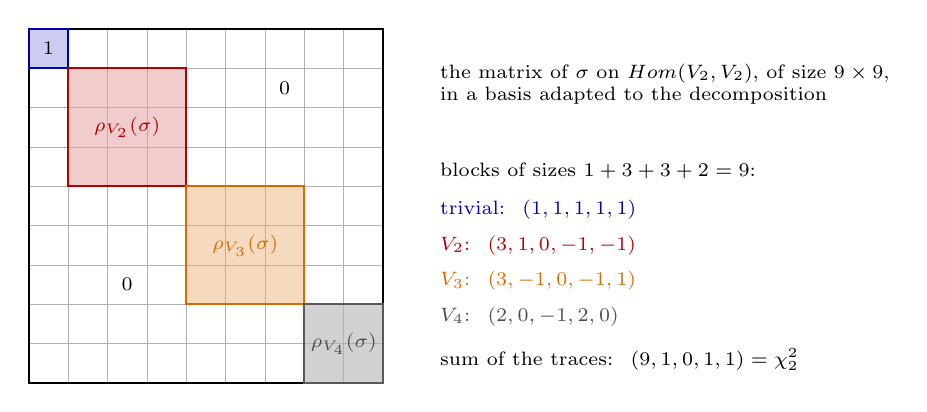
\begin{tikzpicture}[font=\scriptsize, x=0.5cm, y=0.5cm]
\fill[blue!70!black!20] (0,9) rectangle (1,8);
\fill[red!70!black!20] (1,8) rectangle (4,5);
\fill[orange!85!black!25] (4,5) rectangle (7,2);
\fill[black!18] (7,2) rectangle (9,0);
\draw[black!30, very thin, step=1] (0,0) grid (9,9);
\draw[thick] (0,0) rectangle (9,9);
\draw[blue!70!black, thick] (0,9) rectangle (1,8);
\draw[red!70!black, thick] (1,8) rectangle (4,5);
\draw[orange!85!black, thick] (4,5) rectangle (7,2);
\draw[black!65, thick] (7,2) rectangle (9,0);
\node at (0.5,8.5) {$1$};
\node[red!70!black] at (2.5,6.5) {$\rho_{V_2}(\sigma)$};
\node[orange!85!black] at (5.5,3.5) {$\rho_{V_3}(\sigma)$};
\node[black!70] at (8,1) {$\rho_{V_4}(\sigma)$};
\node at (6.5,7.5) {$0$};
\node at (2.5,2.5) {$0$};
\node[anchor=west, align=left] at (10.2,7.6) {the matrix of $\sigma$ on $\operatorname{Hom}(V_2, V_2)$, of size $9 \times 9$,\\in a basis adapted to the decomposition};
\node[anchor=west, align=left] at (10.2,5.4) {blocks of sizes $1 + 3 + 3 + 2 = 9$:};
\node[anchor=west, align=left, blue!70!black] at (10.2,4.4) {trivial: \ $(1, 1, 1, 1, 1)$};
\node[anchor=west, align=left, red!70!black] at (10.2,3.5) {$V_2$: \ $(3, 1, 0, -1, -1)$};
\node[anchor=west, align=left, orange!85!black] at (10.2,2.6) {$V_3$: \ $(3, -1, 0, -1, 1)$};
\node[anchor=west, align=left, black!70] at (10.2,1.7) {$V_4$: \ $(2, 0, -1, 2, 0)$};
\node[anchor=west, align=left] at (10.2,0.6) {sum of the traces: \ $(9, 1, 0, 1, 1) = \chi_2^2$};
\end{tikzpicture}
